\documentclass[a4paper]{article}
\usepackage[margin=1in]{geometry}
\usepackage[english]{babel}
\usepackage[utf8]{inputenc}
\usepackage{amsmath,graphicx,tikz,circuitikz,pgfplots,filecontents,pgfplotstable,booktabs}

\pgfplotsset{compat=1.8}
\usetikzlibrary{decorations.pathmorphing}

\usepackage[justification=centering]{caption}
\usetikzlibrary{arrows,fit,patterns}

\usetikzlibrary{matrix}


\title{Test Document for \LaTeX \ Figures}

\author{Joshua Gruenstein and Michael Truell}

\date{\today}

\begin{document}
	\maketitle

	\section{Figures}
	\centering

	\begin{figure}[ht]
		\centering
		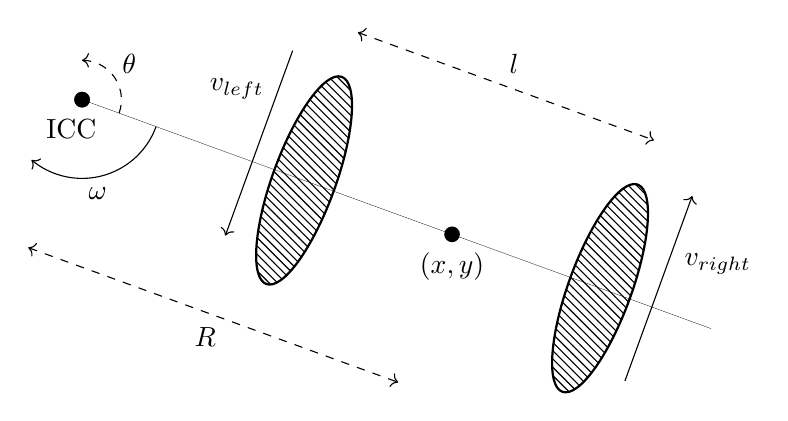
\begin{tikzpicture}
	\begin{scope}[rotate=-20]
		\draw[ultra thin] (0,0) -- (8.5,0);
		\draw[pattern=north west lines,thick](3,0) ellipse (0.4cm and 1.4cm);
		\draw[pattern=north west lines,thick](7,0) ellipse (0.4cm and 1.4cm);

		\node[circle,fill,inner sep=-2pt,label=below:${(x,y)}$] at (5,0){};
		\node[circle,fill,inner sep=-2pt,label={[xshift=.6cm, yshift=0.1cm]$\theta$}] at (0,0){};
		\node[circle,fill,inner sep=-2pt,label={[xshift=.2cm, yshift=-1.5cm]$\omega$}] at (0,0){};
		\node at (0,-.4) {ICC};

		\draw[->,dashed] (.5,0) arc (0:110:.5cm);
		\draw[->] (1,0) arc (0:-110:1cm);

		\draw[->] (2.3,1.5) -- (2.3,-1);
		\node at (1.8,.8) {$v_{left}$};
		\draw[->] (7.7,-1) -- (7.7,1.5);
		\node at (8.3,.8) {$v_{right}$};

		\draw[<->,dashed] (0,-2) -- (5,-2);
		\node at (2.5,-2.3) {$R$};

		\draw[<->,dashed] (3,2) -- (7,2);
		\node at (5,2.3) {$l$};
	\end{scope}

	%\draw[step=.5cm,gray,ultra thin] (-1,1.5) grid (9,-4.5);
\end{tikzpicture}

		\caption{Differential Drive Kinematics}
	\end{figure}

	\begin{figure}[ht]
		\centering
		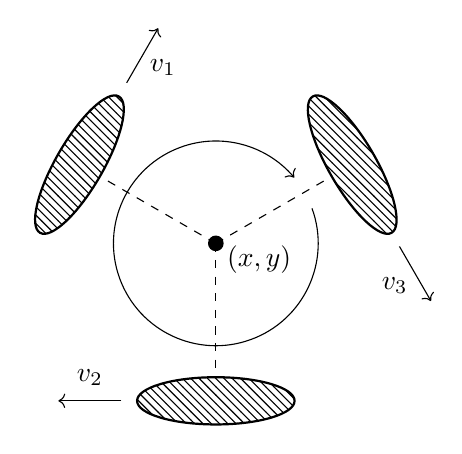
\begin{tikzpicture}
	\node[circle,fill,inner sep=-2pt] at (0,0){};
	\node at (0.55,-0.2) {${(x,y)}$};

	\draw[->,rotate=20] (1.3,0) arc (0:-340:1.3cm);

	\foreach \r [count=\i] in {60,180,300} {
		\begin{scope}[rotate=\r]
			\draw[pattern=north west lines,thick](0,2) ellipse (1cm and 0.3cm);
			\draw[dashed] (0,0) -- (0,1.6);
			\draw[->] (1.2,2) -- (2,2);
			\node at (1.6,1.7) {$v_{\i}$};
		\end{scope}
	};
\end{tikzpicture}

		\caption{Kiwi Drive Kinematics}
	\end{figure}


\end{document}

\end{document}
